%!TEX options=--shell-escape
\documentclass[tikz]{standalone}
\usepackage[T1]{fontenc}
\usepackage[utf8]{inputenc}
\usepackage{xcolor}
\usepackage{amsmath}
\usepackage{amssymb}
\usepackage{hyperref}
\usepackage{accsupp}    
\usepackage{graphicx}
\usepackage{mathtools}
\usepackage{pagecolor}
\usepackage{amsmath} % for \dfrac
\usepackage{tikz}
\tikzset{>=latex} % for LaTeX arrow head
\usepackage{pgfplots} 
\usepackage[edges]{forest}
\usetikzlibrary{patterns, backgrounds, arrows.meta}
\setlength{\parindent}{0cm}
\setlength{\parskip}{1em}
\usepackage{braket}

\usetikzlibrary{patterns}

\begin{document}
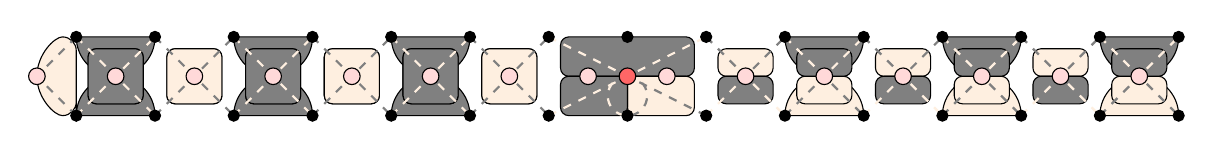
\begin{tikzpicture}[]

 % Plaquettes Left
 \foreach \x in {0, 2,...,4}{
    \draw[black, fill=gray](\x,1) arc (0:180:-0.5) -- cycle;
    \draw[black, fill=gray](\x,0) arc (180:0:0.5) -- cycle;
    } 

   \foreach \x in {0, 2,...,4}{

        \fill[draw=black, fill=gray, rounded corners=3pt] (\x + 0.15, 0.15) rectangle (\x+0.85, 0.85) ;
        \fill[draw=black, fill=yellow!40!red!10, rounded corners=3pt] (\x + 1.15, 0.15) rectangle (\x+1.85, 0.85) ;
    }
    \fill[draw=black, fill=yellow!40!red!10, rounded corners=5pt] (0, 0.1) -- (0, 1) arc (90:270:0.5) -- cycle ;

   % Centralised squares
   \foreach \x in {0, 2,...,4}{
        \fill[draw=black, fill=gray, rounded corners=3pt] (\x + 0.15, 0.15) rectangle (\x+0.85, 0.85) ;
        \fill[draw=black, fill=yellow!40!red!10, rounded corners=3pt] (\x + 1.15, 0.15) rectangle (\x+1.85, 0.85) ;
    }
% Lines
    \foreach \x in {0, 2,...,4}{
           \draw[thick, dashed, gray] (\x+1, 0) -- (\x+2, 1);
           \draw[thick, dashed, gray] (\x+1, 1) -- (\x+2, 0);

           \draw[thick, dashed, yellow!40!red!10] (\x, 0) -- (\x + 1, 1);
           \draw[thick, dashed, yellow!40!red!10] (\x, 1) -- (\x + 1, 0);

    }
           \draw[thick, dashed, gray] (0, 0) -- (-0.5, 0.5);
           \draw[thick, dashed, gray] (0, 1) -- (-0.5, 0.5);




 % Plaquettes Right
 \foreach \x in {9, 11,...,13}{
    \draw[black, fill=gray](\x,1) arc (0:180:-0.5) -- cycle;
    \draw[black, fill=yellow!40!red!10](\x,0) arc (180:0:0.5) -- cycle;
    } 

    % Centralised squares
   \foreach \x in {8, 10,...,12}{
        \fill[draw=black, fill=yellow!40!red!10, rounded corners=3pt] (\x + 0.15, 0.5) rectangle (\x+0.85, 0.85) ;
        \fill[draw=black, fill=gray, rounded corners=3pt] (\x + 0.15, 0.15) rectangle (\x+0.85, 0.5) ;
        \fill[draw=black, fill=yellow!40!red!10, rounded corners=3pt] (\x + 1.15, 0.15) rectangle (\x+1.85, 0.5) ;
        \fill[draw=black, fill=gray, rounded corners=3pt] (\x + 1.15, 0.5) rectangle (\x+1.85, 0.85) ;
    }

    % Merger
        \fill[draw=black, fill=gray, rounded corners=3pt] (6.15, 0.5) rectangle (7.85, 1) ;
        \fill[draw=black, fill=yellow!40!red!10, rounded corners=3pt] (7, 0) rectangle (7.85, 0.5) ;
        \fill[draw=black, fill=gray, rounded corners=3pt] (6.15, 0) rectangle (7, 0.5) ;

        \draw[thick, dashed, yellow!40!red!10] (6, 1) -- (7, 0.5) -- (8, 1);
        \draw[thick, dashed, gray] (8, 0) -- (7, 0.5);
        \draw[thick, dashed, yellow!40!red!10] (6, 0) -- (7, 0.5);

        \draw[thick, dashed, yellow!40!red!10] (7, 0.5) arc (90:270:0.25);
        \draw[thick, dashed, gray] (7, 0.5) arc (270:90:-0.25);


% Lines
    \foreach \x in {8, 10,...,12}{
        \draw[thick, dashed, gray] (\x+1, 0) -- (\x+1.5, 0.5) -- (\x + 2, 0);
           \draw[thick, dashed, yellow!40!red!10] (\x+1, 1) -- (\x+1.5, 0.5) -- (\x + 2, 1);

           \draw[thick, dashed, yellow!40!red!10] (\x, 0) -- (\x + 0.5, 0.5) -- (\x + 1, 0);
           \draw[thick, dashed, gray] (\x, 1) -- (\x + 0.5, 0.5) -- (\x + 1, 1);
    }


        % Dots
    \foreach \x in {0, 1, ...,14}{
           \filldraw[draw=black, fill=black] (\x, 0) circle[radius=2pt] node[font=\tiny] {};
           \filldraw[draw=black, fill=black] (\x, 1) circle[radius=2pt] node[font=\tiny] {};
           \filldraw[draw=black, fill=pink!60] (\x - 0.5, 0.5) circle[radius=3pt] node[font=\tiny] {};
    }
   \filldraw[draw=black, fill=red!60] (7, 0.5) circle[radius=3pt] node[font=\tiny] {};
 


\end{tikzpicture} 
\end{document}

